\section{Correlated Multi-Armed Bandit Model}
\seclabel{background}

Finding an approximate solution of Equation~\ref{eq:objective} using Multi-Armed Bandits requires a predictive model of the probability of force closure for each grasp.
We use Continuous Correlated Beta Processes (CCBPs) to model force closure for a grasp as a Bernoulli random variable with correlations across grasps and objects~\cite{goetschalckx2011continuous, montesano2012active}.
\figref{correlated-motivation} illustrates how using a correlated model can lead to accelerated convergence of bandit algorithms.
%In practice, correlations may occur between two grasps that contact the same shape in similar locations, or between grasps on different shapes, such as grasping the handle of a mug and the handle of a teapot.

\begin{figure}[t!]
\centering
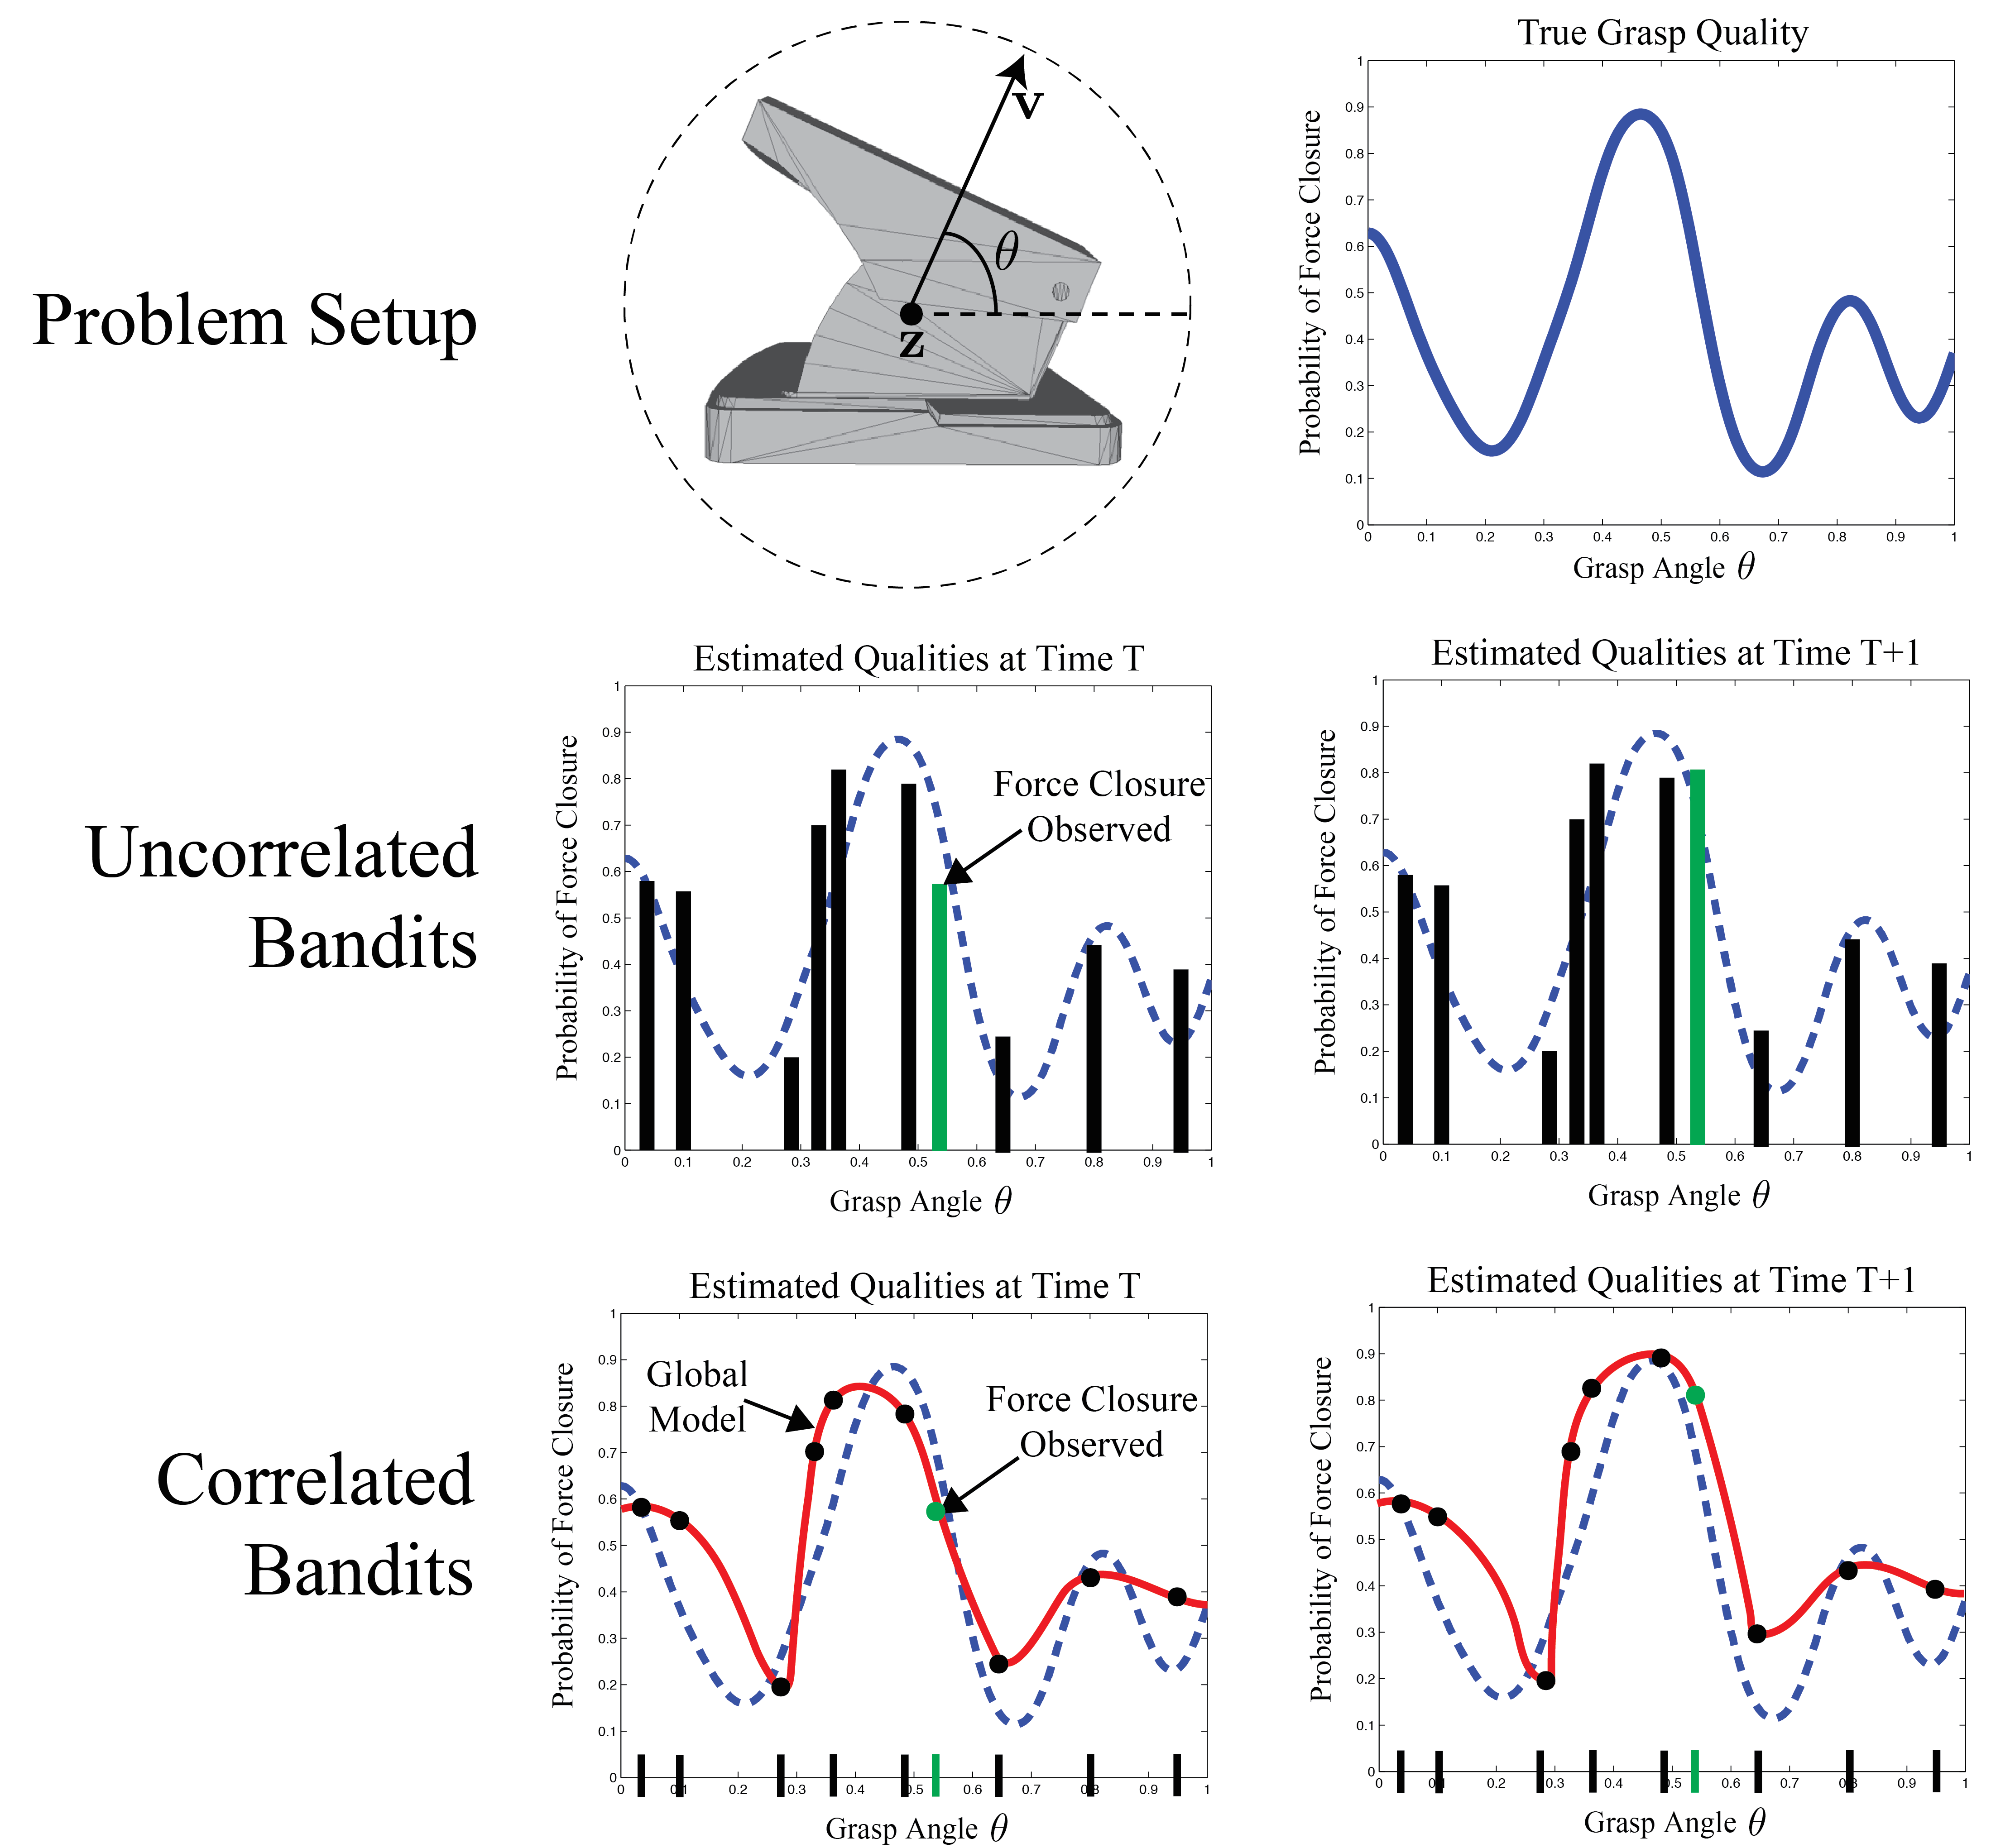
\includegraphics[scale=0.22]{figures/illustrations/correlated_bandits.png}
\caption{(Top Left) Consider a set of grasps with fixed center at an object center of mass and approach direction sampled along a one-dimensional circle. (Top Right) The true probability of force closure $P_F$ may vary smoothly as a function of the angle of the grasp axis. (Middle Left) Uncorrelated MAB models maintain an estimate of $P_F$ independently for each grasp, indicated by bars and their height. On iteration $T$ of a MAB algorithm, the grasp indicated with a green bar is sampled and returns force closure. (Middle Right) Only the estimate of $P_F$ for the sampled grasp is updated for iteration $T+1$, and the grasp with highest estimated $P_F$ remains suboptimal. (Bottom Left) Correlated MAB models maintain a global predictive function (in red) of $P_F$ for any possible grasp but may select grasps from a set of discrete candidates (indicated by dots). (Bottom Right) On iteration $T+1$ the grasp indicated by the green dot again returns force closure and the global model is updated, increasing the estimated $P_F$ for ``nearby" grasps. Although a suboptimal grasp was sampled, the global model now correctly predicts the optimal grasp in the set. }
\figlabel{correlated-model}
\vspace*{-15pt}
\end{figure}

\subsection{Continuous Correlated Beta Processes}

Continuous Correlated Beta Processes(CCBPs) were independently developed by Goetschalckx et al.~\cite{goetschalckx2011continuous} and Montesano and Lopes~\cite{montesano2012active} to model correlations between the Bernoulli random variables in a Beta-Bernoulli process, which may lead to faster convergence in Multi-Armed Bandit problems~\cite{chu2011contextual}.
Such correlations may exist when the Bernoulli random variables depend on common latent factors.
For example, two probability of force closure variables $\theta_k$ may be correlated when two grasps contact the same shape in similar locations or when grasps on different shapes have similar local surface geometries, such as grasping the handle of a mug and the handle of a teapot

Let $\Gamma = \{\bg_k\}_{k=1}^K$ denote our discrete set of $K$ candidate grasps for object $\mO$.
Let $F(\bg_k) \in \{0, 1\}$ denote the occurence of force closure for a grasp $\bg_k$.
We model $F(\bg_k)$ as a Bernoulli random variable with probability of success $\theta_k = P_F(\bg_k)$.
Since we do not know the value of $\theta_k$ for each grasp, we maintain a belief distribution for each $\theta_k$ based on our prior belief about the likelihood of force closure.
A common choice for a belief distribution on the Bernoulli parameter $\theta_k$ is the Beta distribution, which is specified by shape parameters $\alpha > 0$ and $\beta > 0$:

\vspace{-2ex}
\begin{align*}
	\betadist(\alpha, \beta) = \frac{1}{B(\alpha, \beta)} \theta_k^{\alpha-1} (1 - \theta_k)^{\beta-1}
\end{align*}

A CCBP estimates the shape parameters for a grasp $\bg$ on object $\mO$ using a normalized kernel function $k(\by_i, \by_j) : \mM \times \mM \rightarrow [0,1]$ that measures similarity between two elements of the Grasp Moduli Space, where $\by = \{\bg, \mO\} \in \mM$.
The kernel approaches 1 as the arguments become increasingly similar and approaches 0 as the arguments become dissimilar.
In this work we use a unit-bandwidth squared exponential kernel 
\begin{align*}
	k(\by_i, \by_j) &= \exp\left( - \frac{1}{2} \sum \limits_{m=1}^{N_f} w_m^2 \|\phi_m(\by_i) - \phi_m(\by_j)\|_2^2 \right)
\end{align*}
\noindent where $\phi_m: \mM \rightarrow \mathbb{R}^{d_m}$ for $m = 1, ..., N_f$ are feature mappings for a grasp and object to a $d_m$-dimensional Euclidean space and $w_m \in \mathbb{R}$ are weights scaling the relative contribution of the feature maps to the similarity metric.

Upon observing force closure for a grasp and object, we update the Beta belief for every other grasp proportional to how similar it is to the observed grasp as measured by the kernel. 
Let $F_{1}(\bg_{I(1)}), ..., F_{t}(\bg_{I(t)})$ be $t$ sequential observations of force closure from samples of our uncertainty models for grasps $\bg_{I(1)}, ..., \bg_{I(t)}$, where $I(j)$ is the index of the grasp sampled at time $j$.
Then the CCBP posterior update for $\theta_k$ is~\cite{goetschalckx2011continuous}:

\vspace{-2ex}
\begin{align}
	p \left(\theta_k | F_{1}(\bg_{I(1)}), ..., F_{t}(\bg_{I(t)}) \right) &= \betadist\left( \alpha_{k,t}, \beta_{k,t} \right) \notag \\
	\alpha_{k,t} = \alpha_{k,0} &+ \sum \limits_{j=1}^t k(\by_k, \by_{I(j)}) F_{i}(\bg_{I(j)}) \label{eq:alpha} \\
	\beta_{k,t} = \beta_{k,0} &+ \sum \limits_{=1}^t k(g\by_k, \by_{I(j)}) (1 - F_{i}(\bg_{I(j)})) \label{eq:beta}
\end{align}

\noindent Intuitively, this allows observations of one grasp to constitute fractional observations of similar grasps.

\subsection{Feature Mappings}
We use feature mappings $\phi_1, ..., \phi_{N_f}$ that capture both lsimilarity based on local surface geometry and grasp parameters and global object shape.

\subsubsection{Local Features}
Since grasps may be correlated across very small changes to the grasp center and approach direction on a single shape, our first feature map $\phi_{\ell}(\by) = \bg$ is the identity transformation for the grasp.
However, similarity between grasp centers and approach directions does not indicate similar $P_F$ if the two surfaces are dissimilar.
For example, two grasps contacting a box on opposite sides of a corner may be very similar according to $\phi_{\ell}$ but likely to contact the object on surfaces with very different orientations.

To mitigate this issue, we use a variant of the grasp heightmap features of Herzog et al.~\cite{herzog2012template} and Kappler et al.~\cite{kappler2015leveraging}.
In this work, we capture local surface patches by an image oriented along a tangent plane to the grasp axis at a contact point, where each pixel stores the distance from the pixel center on the plane to the surface along the grasp axis.
Let $d_g \in \mathbb{Z}$ be the number of pixels along each dimension of the heightmap, let $\delta \in \mathbb{R}$ be the resolution of the image pixels in meters, and let $r \in \mathbb{R}$ be a minimum projection distance.
Furthermore, let $\bc_k, k = 1, 2$ be a contact point for grasp $\bg$ and let $\bt_1, \bt_2$ be two orthogonal vectors to the grasp approach direction $\bv$.
Then to compute the heightmap value at pixel $(i,j)$ we first compute the 3D location of the pixel on the plane, $\bp_k(i,j) = \bc_k + i \delta \bt_1 + j \delta \bt_2$.
Then we assign the heightmap value $\bh_k(i,j) = t^*$, where $t^*$ is the smallest value of $t > -r$ such that $\bp_k(i,j) + t \bv$ contacts the shape surface.
Finally, we rotate the heightmap to align the axes with the eigenvectors of a weighted covariance matrix as in~\cite{tombariunique} in order to make our feature representation rotationally invariant.
Our feature vector for the heightmaps is $\phi_{h}(\bg_i, \mO_i) = [\bh_1, \bh_2]^T$.
\figref{local-feature-model} illustrates local surface patches extracted by this procedure.

\begin{figure}[t!]
\centering
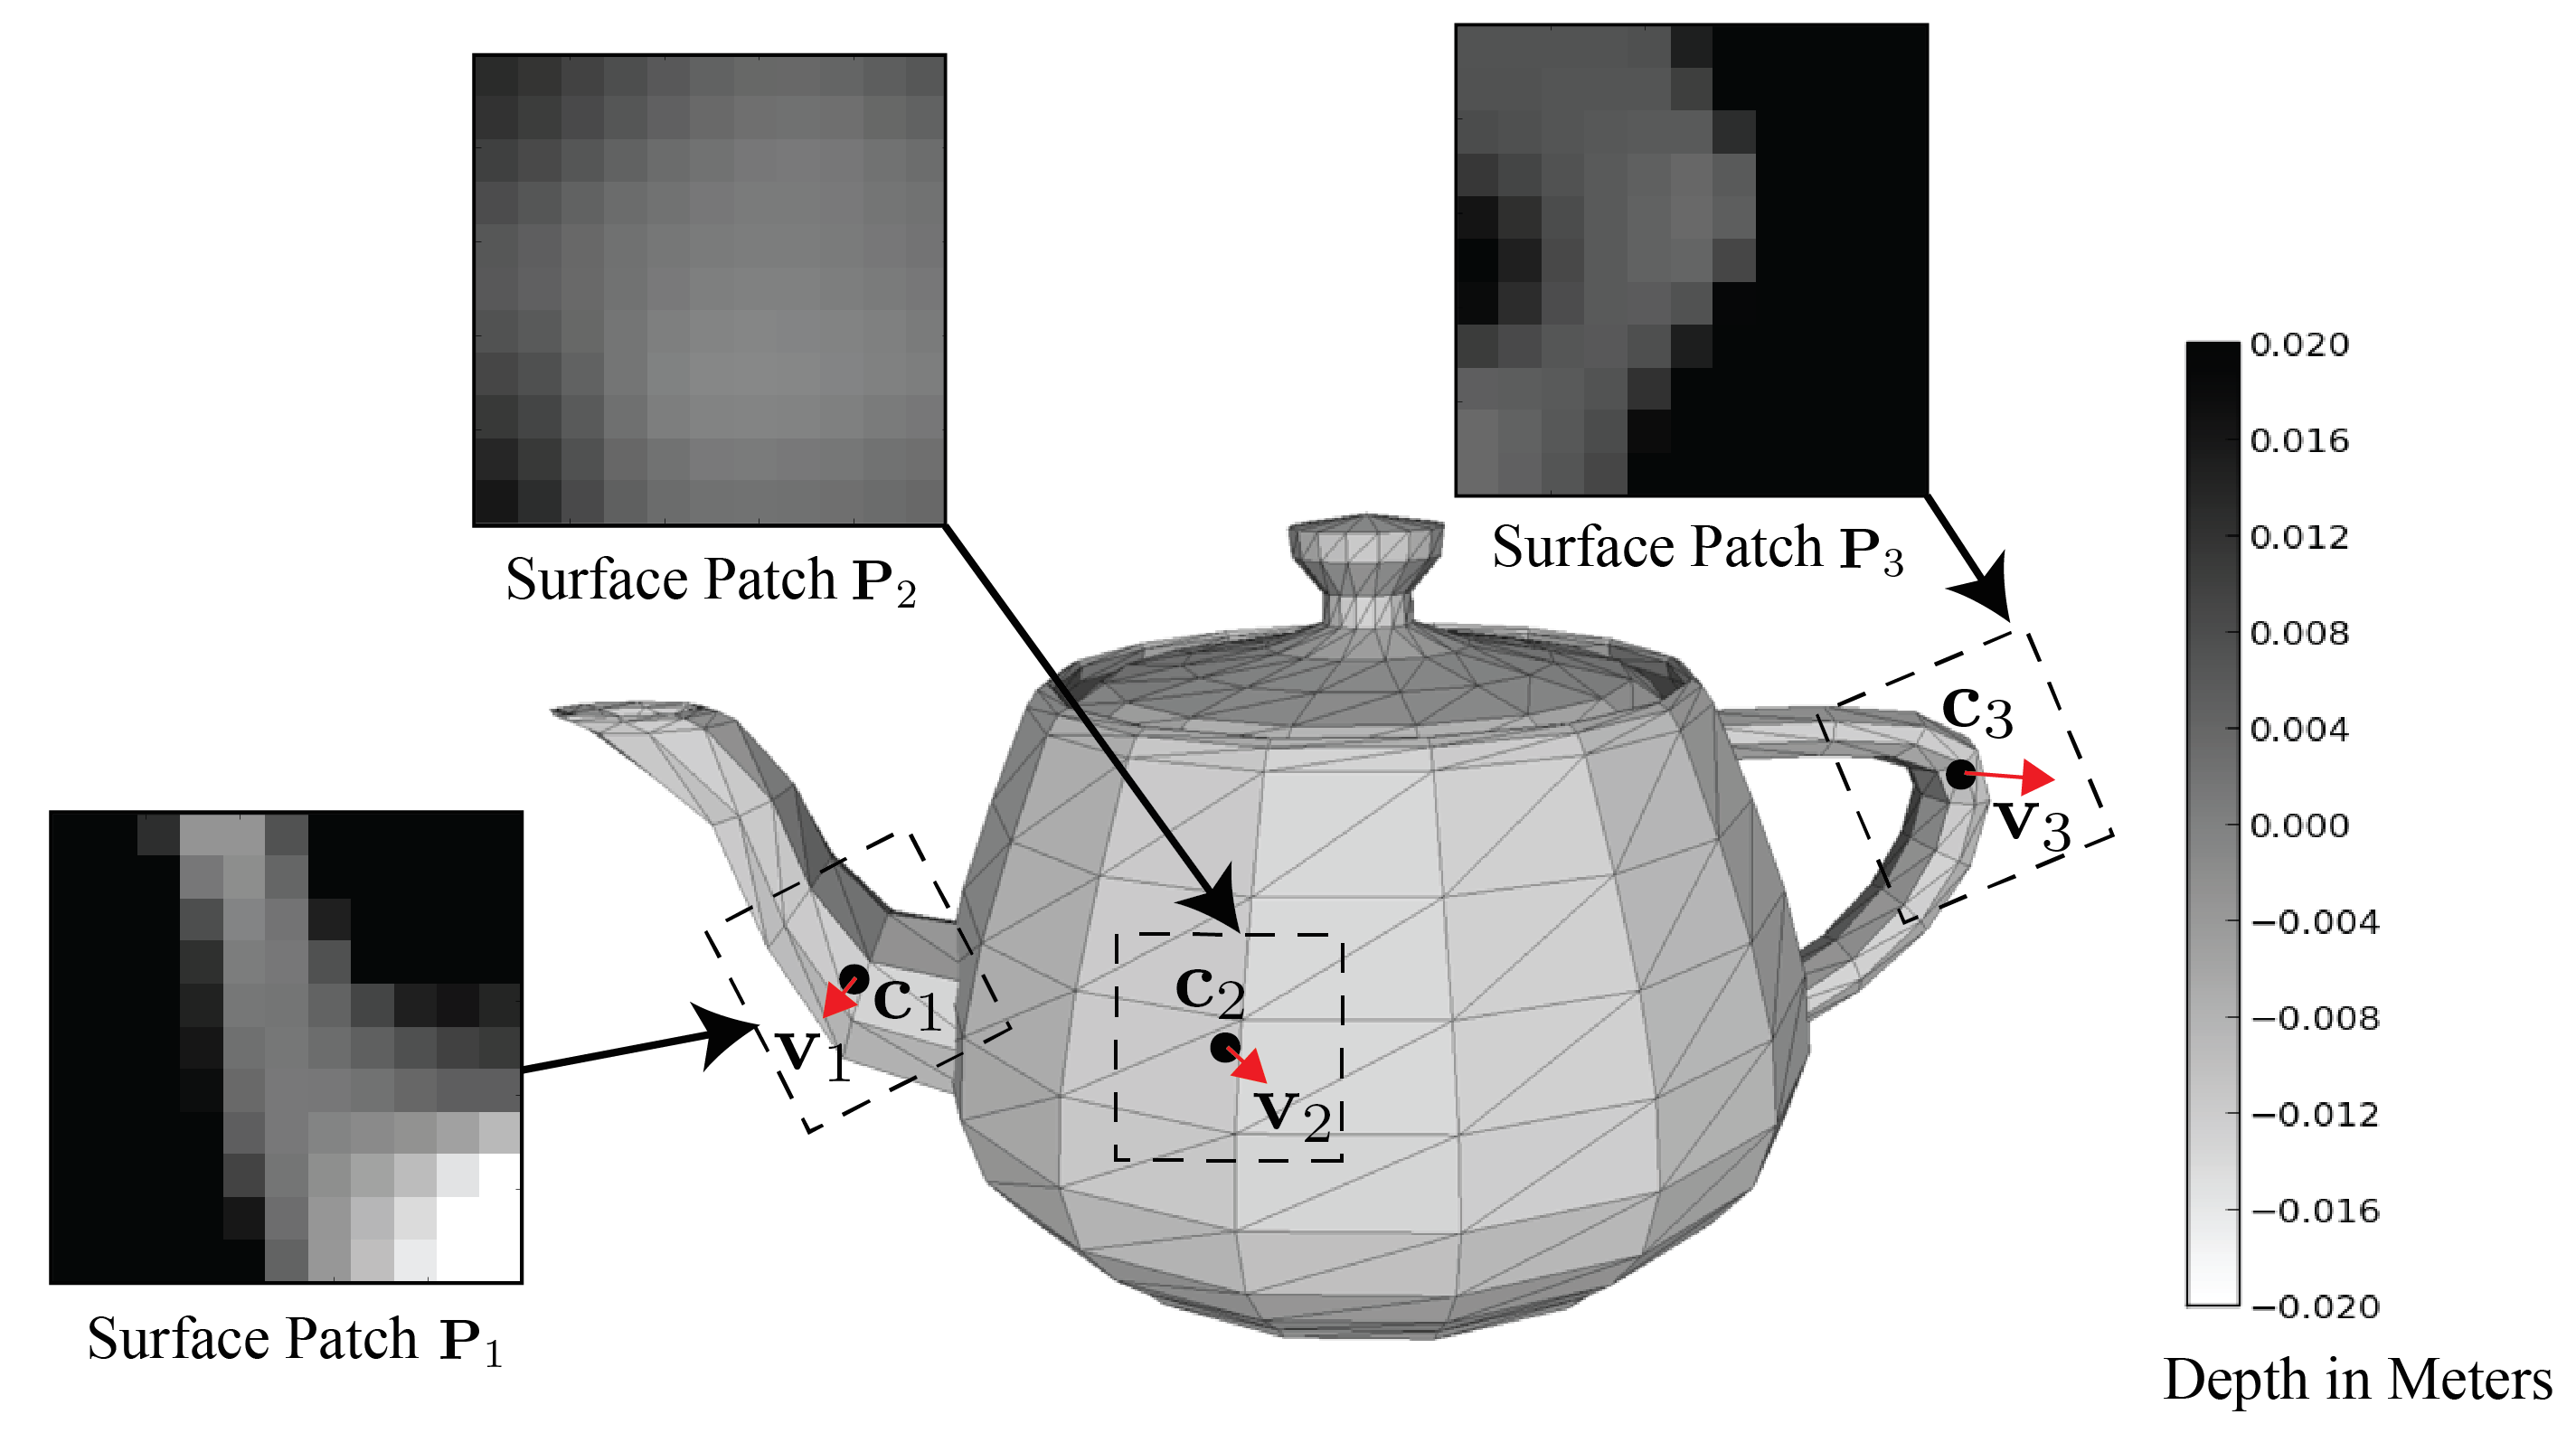
\includegraphics[scale=0.35]{figures/illustrations/local_feature_model.png}
\caption{Three local surface heightmaps extracted on a teapot. Each heightmap is ``rendered" along the grasp axis at each contact point and oriented by the local directions of maximum variation in the heightmap.  }
\figlabel{local-feature-model}
\vspace*{-15pt}
\end{figure}

\subsubsection{Global Features}
Purely local features may not capture all correlations in probability of force closure between pairs of grasps and objects.
For example, grasps on the handle of a teapot may have similar grasp center, grasp axis, and even local surface geometry to another tubelike object such as a pen, but different $P_F$.
To measure global shape similarity, we develop a novel viewpoint-based object representation that pools the views from many virtual viewpoints rendered on a sphere surrounding the object.

\TODO{Justify why class labels help, if they do}
\figref{global-feature-model} illustrates our method.
We first render every object to 50 virtual cameras discretized along equal angle increments and oriented toward the object center using Maya.
Then we finetune AlexNet~\cite{krizhevsky2012imagenet}, a common deep Convolutional Neural Network (CNN) architecture, to predict a class label for each image based on known class labels for the 3D models.
%While class labels are not necessarily indicative of similarity in the geometry relevant to grasping, in many cases the same class label is enough to guarantee some correspondence of global geometry.
Next, we pass each of the 50 views of each object through the finetuned CNN and max-pool the output of the fc7 layer.
As the output is nearly 400 dimensions, we finally reduce the max-pooled output to 100 dimensions using Principal Component Analysis (PCA).
This yields a representation $\psi(\mO) \in \mathbb{R}^{100}$ for each object.

\TODO{Expand above paragraph, include more details on method as well as the results of training}

\begin{figure}[t!]
\centering
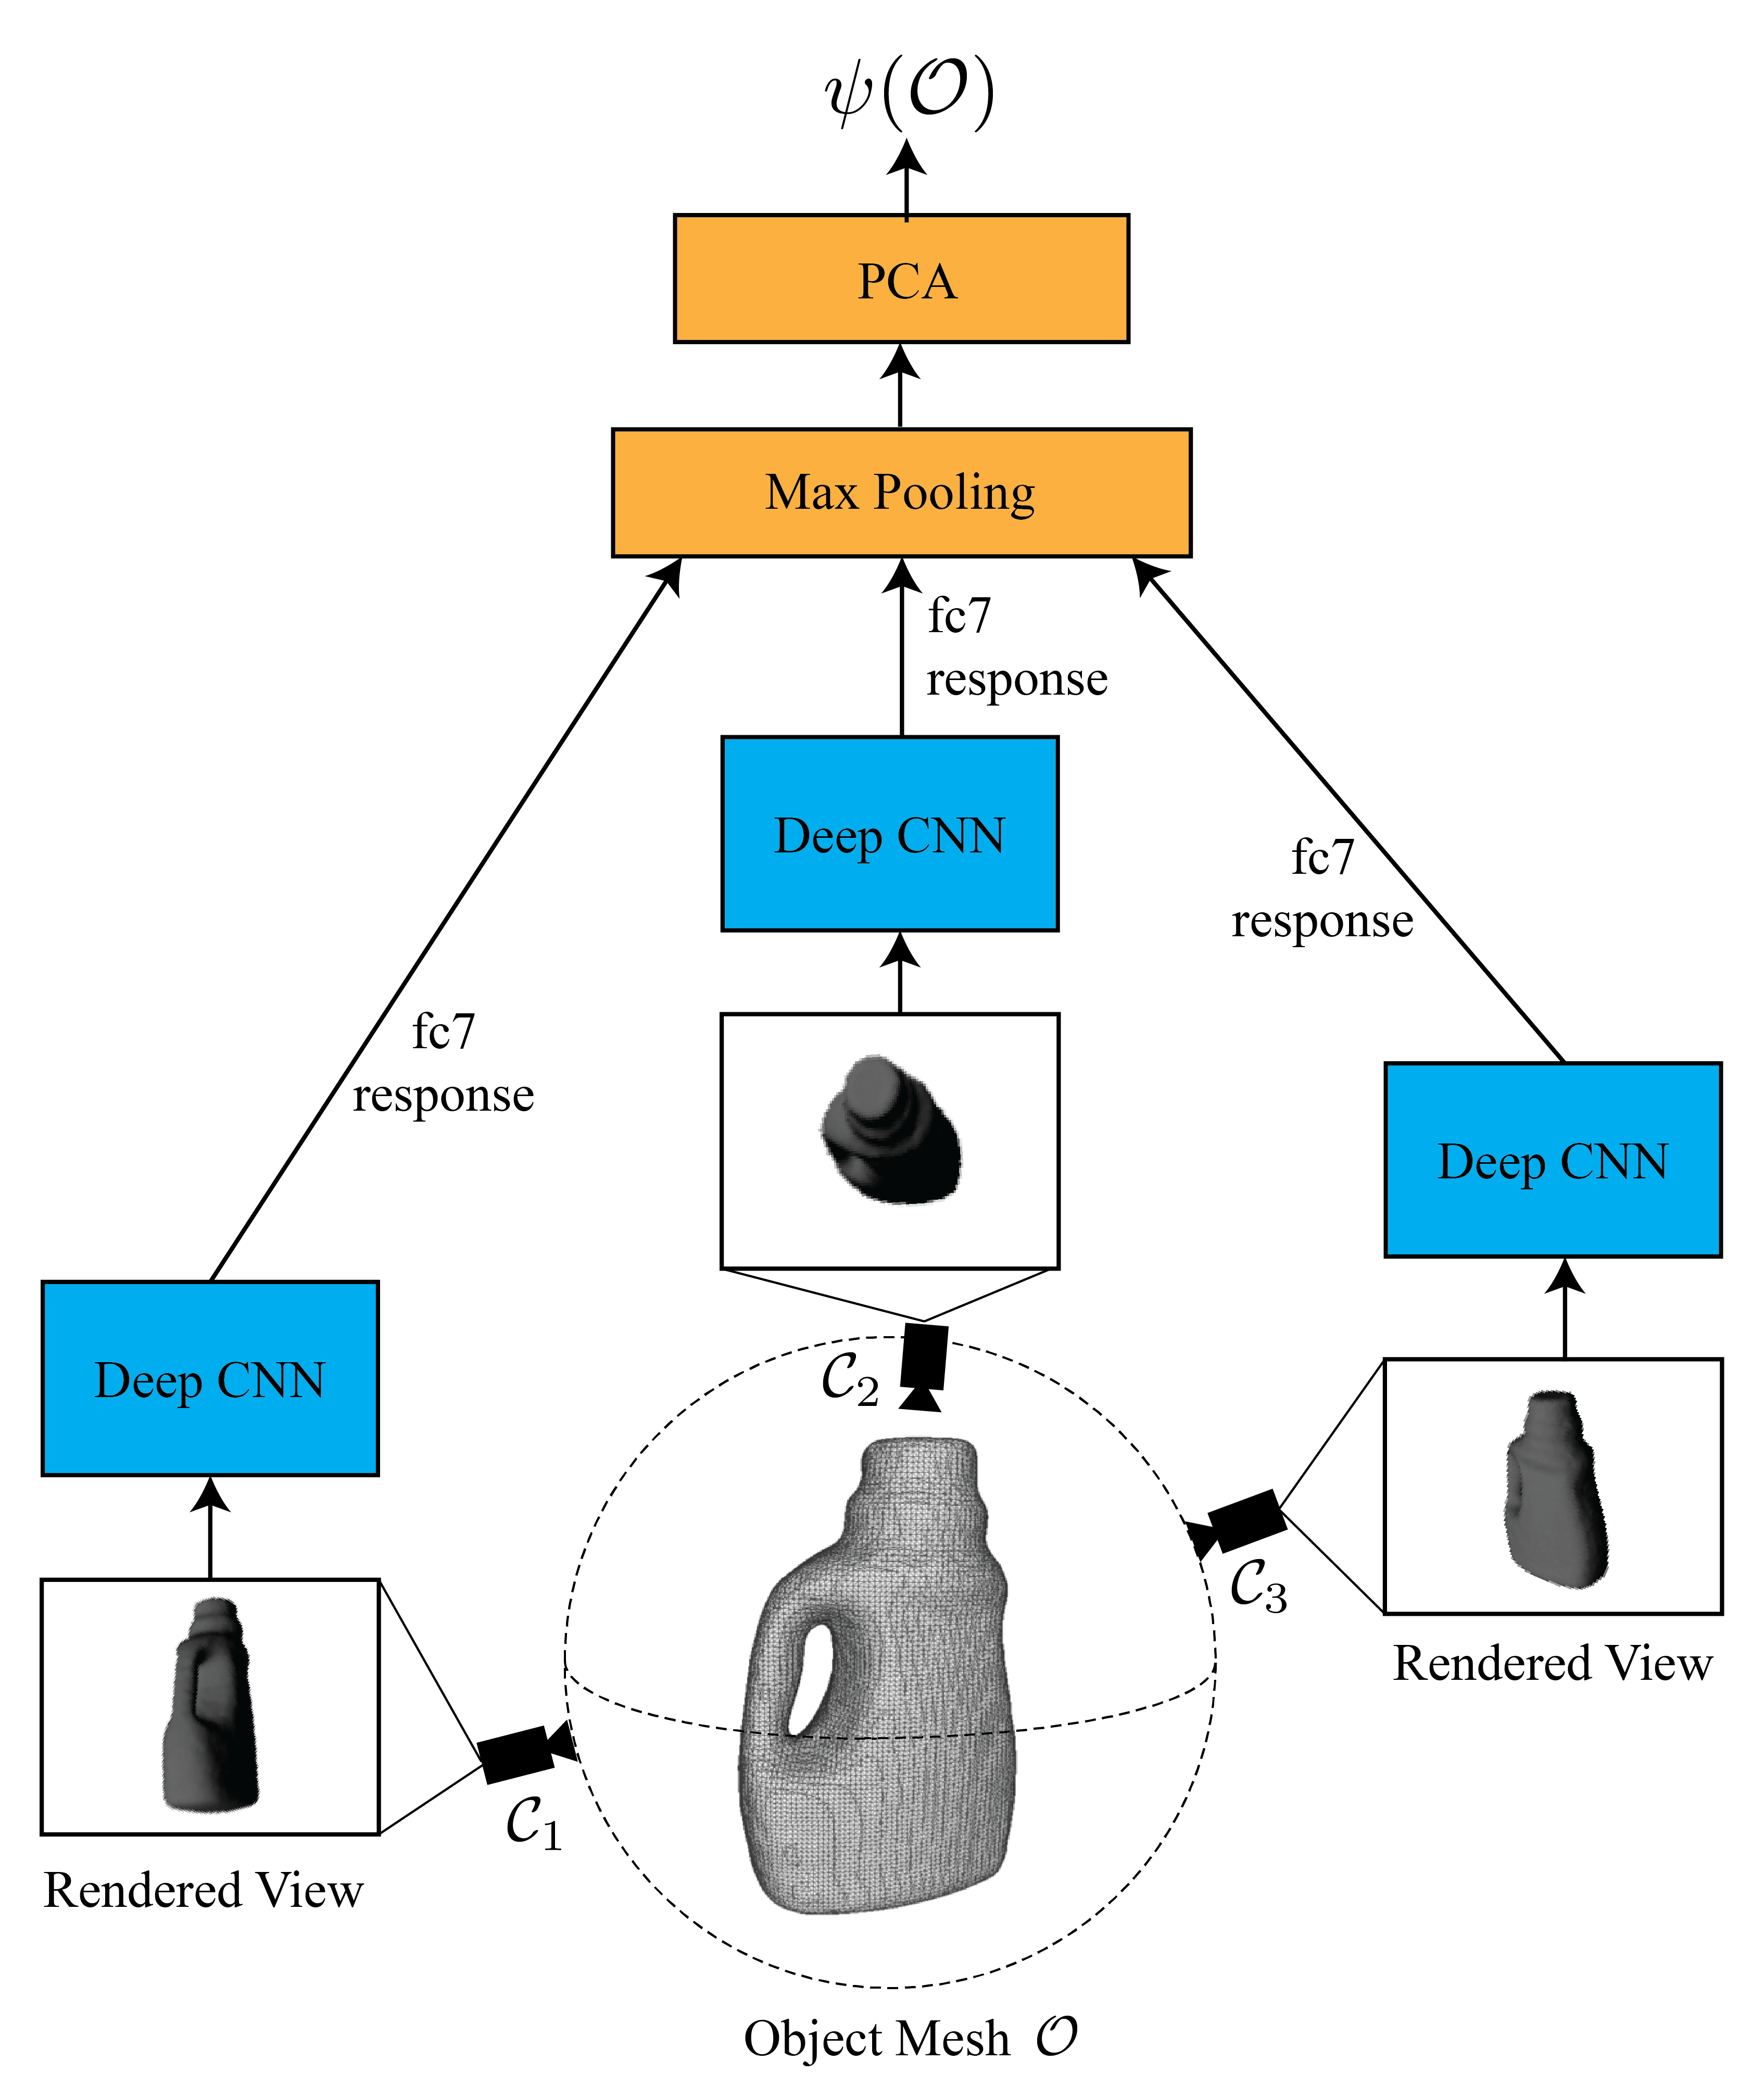
\includegraphics[scale=0.3]{figures/illustrations/cnn_model.png}
\caption{Illustration of our method for embedding 3D object models in a Euclidean vector space for computing global shape similiarty. We pass a set of 50 virtually rendered camera viewpoints discretized around a sphere through a deep Convolutional Neural Network (CNN) with the AlexNet~\cite{krizhevsky2012imagenet} architecture. Finally, we take the maximum fc7 response across each of the 50 views for each dimension and run PCA to reduce the dimensionality of the output.}
\figlabel{global-feature-model}
\vspace*{-15pt}
\end{figure}

\subsection{Optimizing Feature Weights}
One remaining issue is the selection of the relative feature weights $w_1, ..., w_{N_f}$.
Past work has optimized these weights using a squared error loss on the probability of success predicted by the CCBP and a true probability of success from brute force evaluation~\cite{montesano2012active}.
However, this criterion may be inappropriate for predicting probabilities, as the predictions must be bounded between 0 and 1.
In this work we instead select the weights which minimze the cross entropy loss~\cite{}:

\begin{align*}
	w_1^*, ..., w_{N_f}^* = \myargmin{w_1 \geq 0, ..., w_{N_f} \geq 0} \frac{1}{M} \sum \limits_{i=1}^M &\mu_i \log \left( \frac{\alpha_i}{\alpha_i + \beta_i} \right) + \\  &(1 - \mu_i) \log \left( \frac{\beta_i}{\alpha_i + \beta_i} \right)
\end{align*}
\noindent where $\alpha_i$ and $\beta_i$ are the posterior shape parameters given by Equations~\ref{eq:alpha} and~\ref{eq:beta} and $\mu_i$ is the known probability of force closure evaluated by exhaustive Monte-Carlo integration for a set of $M$ grasps.
We optimize this objective using Stochastic Gradient Descent (SGD) with the weights all initialized to 100.